\documentclass[10pt,a4paper]{article}
\usepackage[latin1]{inputenc}
\usepackage{amsmath}
\usepackage{amsfonts}
\usepackage{amssymb}
\usepackage{float}
\usepackage{listings}
\usepackage{graphicx}
\usepackage{subfig}
\usepackage{caption}
\usepackage[usenames,dvipsnames]{color}
\usepackage{fullpage}

\begin{document}
\definecolor{light-gray}{gray}{0.90}
\lstset{language=Python,breaklines=true,backgroundcolor=\color{white},frame=single,showspaces=false,showstringspaces=false,showtabs=false}
\captionsetup{width=10.0cm}

\author{Jeroen Hofman\\
		10194754\\
		}
\title{Disease spreading on small-world networks\
		}
\maketitle

\begin{center}
\abstract{
\noindent In this report we investigate disease spreading on small-world networks. First we investigate properties of small-world networks and examine two types of disease spreading models, SIR and SIRS. We find that the disease spreading rate on a SIR model scales with the average path length of the network. Furthermore we examine state synchronization of the SIRS model after reaching the equilibrium state. The state synchronization increases with increasing rewire probability $p$ and an order parameter can be defined to find the critical point at which the unsynchronized states become synchronized. The critical point is $p \approx 0.15$. The phase transition seen by means of the order parameter can be explained by a rapidly decreasing clustering coefficient and a large spreading in the distribution of local clustering coefficients in the critical area.}
\end{center}

\newpage
\tableofcontents
\newpage

\section{Theory}
\subsection{Construction of small-world networks}
\noindent In 1998 Watts and Strogatz invented an algorithm which generates graphs which are neither fully regular nor fully random \cite{Watts Strogatz}. One starts with a fully regular ring graph consisting of $N$ nodes, where each node has $K$ neighbors, $K/2$ on each side, with $K >> \text{log}N$ \cite{paper3}. One then defines a special parameter $0 < p < 1$, called the rewiring probability. Next one considers every edge of the regular graph and rewires the edge with probability $p$ (i.e. keeping one side fixed and connecting the other side to another node). For small values of $p$ this creates a graph which has retained the structure of the original regular graph, but with additional shortcuts. For values of $p$ close to 1 almost all edges are rewired and the graph becomes nearly random. See figure \ref{fig:smallworld} for a graphical interpretation of the algorithm.\\

\begin{figure}[H]
  \centering
  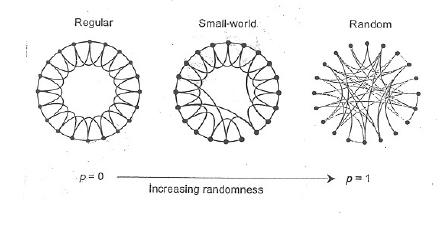
\includegraphics[scale=1.0]{smallworld.jpg}
  \caption{Graphical interpretation of the above algorithm. Starting from a regular network (left) and rewiring connections gives a small-world network (middle). If the rewiring probability is 1 a graph similar to a random graph is obtained (right).}
  \label{fig:smallworld}
\end{figure}

\noindent To analyse the structure of a graph two parameters are used; the average path length L($p,K$) describing the average node-to-node distance between any two nodes on the graph and the clustering coefficient C($p,K$), which is the sum of the local clustering coefficients c$_{i}(p,K)$:
\begin{equation}
C(p,K) = \frac{1}{N} \sum_{i = 1}^{N} \text{c}_{i}(p,k)
\end{equation}
where
\begin{equation}
\text{c}_{i}(p,K) = \frac{\text{\# connections between neighbors of i}}{\text{max \# connections between neighbors of i}}
\end{equation}
where the maximum number of connections between $k$ neighbors is equal to $\frac{k(k-1)}{2}$. These parameters can be calculated for specific values of $p$ with a fixed $K$, in figure \ref{fig:lpcp} L($p$) and C($p$) are plotted for different values of $0 < p < 1$ with $K = 5$ and $N = 1000$, averaged over 100 realizations per $p$ value.\\

\begin{figure}[H]
  \centering
  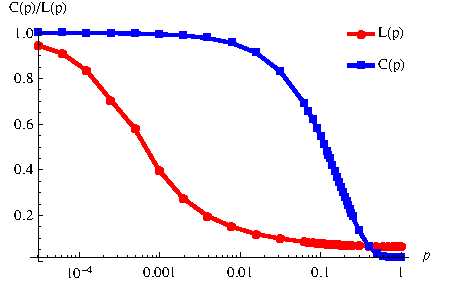
\includegraphics[scale=1.1]{lpcp.pdf}
  \caption{The average path length L$(p)$ and the clustering coefficient C$(p)$ as a function of $p$.}
  \label{fig:lpcp}
\end{figure}

\noindent From figure \ref{fig:lpcp} it is seen that the average path length decreases very rapidly with increasing $p$, whereas the clustering coefficient only starts decreasing with high values of $p$. Regular graphs (i.e. $p \approx 0$) have a high clustering coefficient because the graph is essentially one big cluster, and a high average path length because the graph contains no shortcuts. Random graphs ($p \approx 1$) have a low clustering coefficient, because the random edges prevent formation of clusters, and a low average path length because there is an abundance of shortcuts. The area in between, where C($p$) is high but L($p$) is low is the area in which networks are called small-world networks. Small-world networks resemble many real networks, e.g. social networks, neural networks or distributing networks. A study made in reference \cite{Watts Strogatz} indeed shows that many real life networks fall in the category of small-world networks.

\subsection{Disease spreading models}
\noindent In this paper we study two different types of disease spreading on networks, called SIR and SIRS, where the latter is an extension of the former \cite{paper1}. Starting with a network, we can assign three possible states to every node, susceptible (S), infected (I) and recovered (R), coupled to a disease cycle time counter, which is different for every node. For the SIR network the following relations are defined for the time counter $\tau_{i}$ and state $\pi_{i}$ of node $i$ for universal time $t$:
\begin{eqnarray}
\pi_{i}(t) = \text{S} \; \text{if} \; \tau_{i}(t) = 0 \\
\pi_{i}(t) = \text{I} \; \text{if} \; 1 \leq \tau_{i}(t) < t_{\text{inf}} \\
\pi_{i}(t) = \text{R} \; \text{if} \; \tau_{i}(t) = t_{\text{inf}} 
\end{eqnarray}
where $t_{\text{inf}}$ is the amount of time steps an infected node stays infected. The evolution of the system obeys the following rules:
\begin{eqnarray}
\tau_{i}(t+1) = 0 \; \text{if} \; \tau_{i}(t) = 0 \; \text{and no infection occurs}\\
\tau_{i}(t+1) = 1 \; \text{if} \; \tau_{i}(t) = 0 \; \text{and node i becomes infected}\\
\tau_{i}(t+1) = \tau_{i}(t) + 1 \; \text{if} \; 0 < \tau_{i}(t) < t_{\text{inf}}\\
\tau_{i}(t+1) = \tau_{i}(t) \; \text{if} \; \tau_{i}(t) = t_{\text{inf}}
\end{eqnarray}
We can modify the above schemes to allow a node in the R state to jump back to the S state after a number of steps $t_{\text{rec}}$, thus creating a loop for every node of $t_{\text{inf}} + t_{\text{rec}}$ steps:
\begin{eqnarray}
\pi_{i}(t) = \text{S} \; \text{if} \; \tau_{i}(t) = 0 \\
\pi_{i}(t) = \text{I} \; \text{if} \; 1 \leq \tau_{i}(t) < t_{\text{inf}} \\
\pi_{i}(t) = \text{R} \; \text{if} \; t_{\text{inf}} \leq \tau_{i}(t) < (t_{\text{inf}} + t_{\text{rec}}) 
\end{eqnarray}
and corresponding rules:
\begin{eqnarray}
\tau_{i}(t+1) = 0 \; \text{if} \; \tau_{i}(t) = 0 \; \text{and no infection occurs}\\
\tau_{i}(t+1) = 1 \; \text{if} \; \tau_{i}(t) = 0 \; \text{and node i becomes infected}\\
\tau_{i}(t+1) = \tau_{i}(t) + 1 \; \text{if} \; 0 < \tau_{i}(t) < (t_{\text{inf}} + t_{\text{rec}})\\
\tau_{i}(t+1) = 0 \; \text{if} \; \tau_{i}(t) = (t_{\text{inf}} + t_{\text{rec}})
\end{eqnarray}
From the above rules it follows that the SIR model reaches a steady state when all the nodes are either in state S or state R, because there will be no infected nodes after a certain time. For SIRS however, the process can go on indefinitely and, according to the parameters of the model, can exhibit various types of behavior as we will see in the next section.

\section{Analysis}
\subsection{Spreading rates}
\noindent The SIR model described in the previous section can be used to analyze the behavior of the spreading of diseases in the initial stage of infection, where we assume that the disease can spread uninhibited. In particular two properties can be defined, $r_{1/2}$ and $r_{\text{total}}$, which describe the number of steps before the disease has infected half the number of nodes or all the nodes respectively. Figure \ref{fig:r} shown below shows $r_{1/2}$ and $r_{\text{total}}$ as a function of $p$ for $N = 1000$, $K = 5$, $t_{\text{inf}} = 4$ and $p_{\text{inf}} = 1.0$ (the probability of infection), averaged over 100 realizations per $p$ value. The number of steps needed for both halve and full penetration decreases rapidly for increasing $p$ following the characteristic shape of the L$(p)$ curve. Hence the disease spreading scales with the average path length and so for the small-world networks, which are in a region of low average path length, disease spreading will be nearly as fast as for random networks. Secondly the difference between full and half penetration is small for fixed $p$, which is expected for an infection probability of 1. This is because when half of the nodes is infected, the rest of the network will be infected within a few time steps, because neighbors of infected nodes will become infected with probability 1.

\begin{figure}[H]
  \centering
  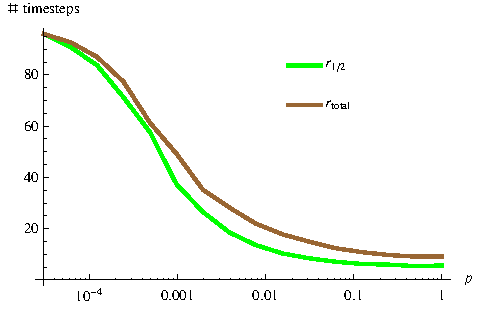
\includegraphics[scale=1.1]{r.pdf}
  \caption{The spreading time for the disease when it has infected half of the graph ($r_{1/2}$) and when it has infected the full graph ($r_{\text{total}}$) as a function of $p$.}
  \label{fig:r}
\end{figure}

\subsection{Equilibrium states}
\noindent After the initial disease spreading the disease can reach an equilibrium state, which can be modelled using the SIRS model (the SIR model also reaches an equilibrium state, but this is the uninteresting case where all nodes have recovered). In the SIRS model first the disease spreading goes exponentially like the case we analysed in the previous section, but as soon as nodes start transforming from the recovered state to the susceptible state again it allows for the occurence of some oscillatory behavior. Figure \ref{fig:p} shows the behavior of the number of susceptible, infected and recovered nodes when the system has reached equilibrium as a function of time, for $p = 2^{-12}, p = 2^{-5}$ and $p = 1$. The parameters used are $N = 1000$, $K = 5$, $p_{\text{inf}} = 0.1$, $t_{\text{inf}} = 8$ and $t_{\text{rec}} = 8$.
 
\begin{figure}[H]
 \centering  
 \subfloat{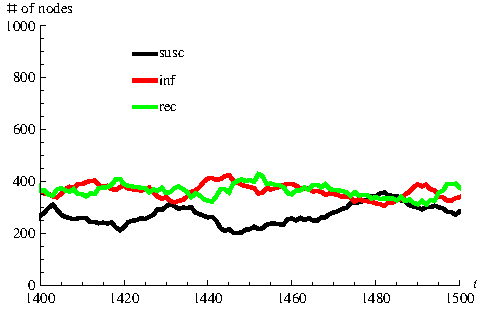
\includegraphics[width=0.33\textwidth]{periodlowp.pdf}}
 \subfloat{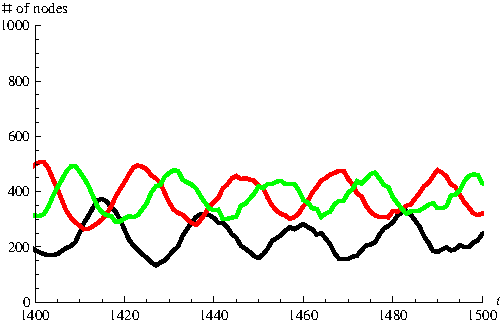
\includegraphics[width=0.33\textwidth]{periodmidp.pdf}}
 \subfloat{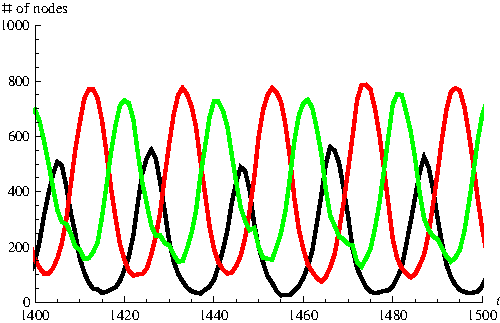
\includegraphics[width=0.33\textwidth]{periodhighp.pdf}}
 \caption{Evolution in time of the number of susceptible, infected and recovered nodes for $p = 2^{-12}$, $p = 2^{-5}$ and $p = 1$.}
 \label{fig:p}
\end{figure}

\noindent The higher the value of $p$ the more there seems to be an oscillatory behavior (we will make this more precise below). Furthermore the period of the oscillations seen in the two figures on the right is bigger than $t_{\text{inf}} + t_{\text{rec}}$, namely 22.2 and 20.4 respectively, which is understandable since the system cannot oscillate faster than 1 cycle time takes and the higher $p$ is the more the average path length decreases, which will increase the rate at which the states can be synchronized over the whole network. The figure below also shows this, giving the oscillation period as function of $p$ obtained by fitting a cosine to the data. Indeed the oscillation period decreases for increasing $p$. 

\begin{figure}[H]
  \centering
  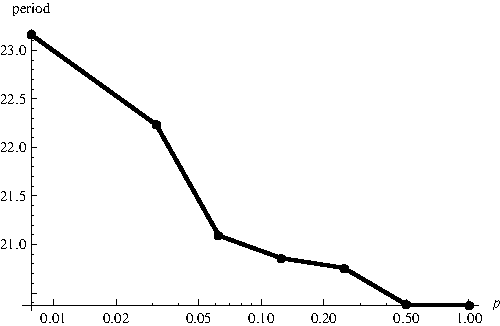
\includegraphics[scale=1.1]{period.pdf}
  \caption{Some values of the oscillation period as a function of $p$, determined by fitting a cosine to the data.}
  \label{fig:sigma}
\end{figure}

\noindent Though for all values of $p$ there is an equilibrium state the system only starts oscillating for high values of $p$, which can be explained by small average path lengths which ensure fast synchronization of nodes over the network.\\
The synchronization of states can be made more precise by using an order parameter \cite{paper4}, defined by:
\begin{equation}
\sigma (t) = \mid \frac{1}{N} \sum_{i = 1}^{N} e^{i \phi_{i} (t)} \mid \; \text{with} \; \phi_{i} (t) = 2 \pi \frac{\tau_{i}(t) - 1}{t_{\text{inf}} + t_{\text{rec}}}
\end{equation}
where the case $\tau_{i}(t) = 0$ is not included, because this time state is overrepresented. For low values of $p$ the states are unsynchronized and so $\sigma(t)$ will be close to 0, for high values of $p$ however the states are more synchronized and so $\sigma(t)$ will not be close to zero anymore. Figure \ref{fig:sigma} below shows $\sigma$ for different values of $p$, averaged over time (2000 time steps) and 50 realizations per $p$, using the same parameters as before. 

\begin{figure}[H]
  \centering
  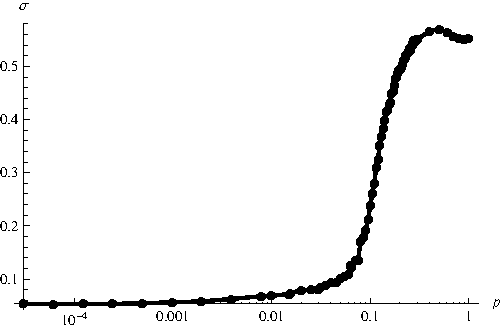
\includegraphics[scale=1.1]{sigma.pdf}
  \caption{$\sigma$, the order parameter as a function of $p$.}
  \label{fig:sigma}
\end{figure}

\noindent The figure shows a steep increase of $\sigma$ around $p = 0.15$, indicating that the system goes from an unsynchronized state to a synchronized one around this value. If we compare this with the clustering coefficient in figure \ref{fig:std} it is seen that the increase of $\sigma$ is in the same region as where the clustering coefficient goes from high values to low values. We can try to understand this phase transition better by also analyzing the standard deviation of the local clustering coefficient $\text{c}_{i}(p)$, which gives a measure of the width of the distribution of local clustering coefficients, and which peaks around the same value as where the derivative of $\sigma(p)$ peaks, see figure \ref{fig:std} below. The spreading of the local clustering coefficient is large around $p = 0.15$, indicating that there are both highly clustered regions and lowly clustered regions around this value of $p$. For low values of $p$ the standard deviation is small and the clustering coefficient is high, so there are many big clusters, for high values of $p$ de standard devation is again small but the clustering coefficient is low, so there are no big clusters anymore. Hence the phase transition can be linked to the clustering coefficient, with an intermediate phase in the small-world domain where the clustering coefficient decreases as a function of $p$ and the ordering parameter increases as a function of $p$, coupled to a large distribution in local clustering coefficients.

\begin{figure}[H]
  \centering
  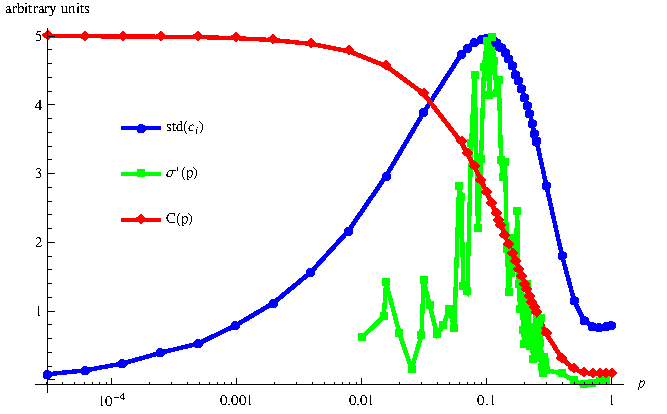
\includegraphics[scale=0.7]{std.pdf}
  \caption{The standard deviation of the local clustering coefficient, the derivative of $\sigma$ and the clustering coefficient C($p$) all shown together.}
  \label{fig:std}
\end{figure}

\section{Conclusion and discussion}
We investigated behavior of small-world networks, constructed by an algorithm designed by Watts and Strogatz in the late 90's. Small-world networks typically have a large clustering coefficient but a small average path length. Small-world networks can be used to model disease spreading, which we did using the SIR and the SIRS model. With the SIR model the disease spreading was investigated, which turns out to scale with the average path length. With the SIRS model we studied the occurence of state synchronization as a function of $p$. We defined an order parameter and found the phase transition from unsynchronized to synchronized states to be at $p \approx 0.15$, which coincides with the region of rapidly decreasing clustering coefficient and high values of the standard deviation of the local clustering coefficient. Hence this transition region seems to be corresponding to local high clustering and local low clustering regions across the network.\\
\\
\noindent The validity of these kind of models is still an ongoing debate. Especially when the nodes are interpreted as humans the question arises whether static nodes (with static edges) represent a realistic model, since in real social networks connections change rapidly and constantly \cite{paper2}. It depends on the infection rate of the disease whether or not the static model is realistic. For low infection rates, people will not get infected after one isolated contact but will more probably be infected by their regular contacts, hence a model where each edge can be given a weight (according to the amount of social interaction between two persons) would be a realistic in such a case. For highly infectious diseases the single contacts (for instance in public transport) become very important.
Another important aspect is that the parameters that are used in the model might not be constant, because the disease may evolve or the nodes might start behaving differently. Especially when investigating disease spreading on social networks the behaviour of humans should be taken into account, because people might start taking precautions after the disease has spread to a significant part of the population for example.
Furthermore the analytical background for these types of networks which are neither regular nor random is still very poor and much theoretical work has yet to be done. There are examples of very simple onedimensional directed percolation models (which is basically a simplification of a network one dimensional line) obeying very simple rules which are not yet analytically solvable, so there is still a long way to go in the theoretical field of this subject.

\section{Methods and learning process}
In this section I describe the tools I used and the knowledge I have obtained via this project. As can be seen in the attached source code I have programmed my code entirely in PYTHON, since that was one of my learning goals. In PYTHON I used the package IGRAPH, which provides functions to make graphs and also provides functions to plot graphs and to animate graphs. Most of the figures in this report however are made in Mathematica, which was a tool I used before and now I have refreshed my knowledge concerning this program, using it mostly for my graphical output. Almost all of the editing and coding (including writing this report) is done in EMACS, which I started using at the beginning of the project.\\
As described in the report I used stochastic models to describe disease spreading. It is also possible to write down a system of coupled ODE's and solve this system using some particular solvers, like Runge-Kutta methods. However, in the early stages of the project I choose a topic about enzyme kinetics, which involved solving a system of coupled ODE's, which turned out to be very simple to program and not add much to my programming knowledge. I found this topic to be very interesting and insightful and it was fun to learn PYTHON and some stochastic modelling. I am looking forward to the next obligatory course of the programme, Stochastic Simulation, which will hopefully give a more broad overview of the field of stochastics.\\
I choose this particular topic because I have done some very simple simulations on directed percolation disease models before and I found that to be very interesting. My main interests at the moment lies in the area of complex dynamical systems, where this subject can also be classified under, so this project was an excellent way in getting more familiar with these kind of systems.\\
My starting point for the literature was the paper published by Watts and Strogatz about the dynamics of small-world networks. Than I looked at papers using the small-world algorithm to construct such networks and do some analysis on them. Next to the papers cited in the bibliography I used various Wikipedia pages on topics related to small-world networks. There are many papers on this topic and most of them are still fairly recent, showing that this is an active research area.

\begin{thebibliography}{5}
\bibitem{Watts Strogatz}
  Watts, Duncan J.; Strogatz, Steven H.., \emph{Collective dynamics of 'small-world' networks}, Nature, 6/4/98, Vol. 393 Issue 6684, p440
\bibitem{paper1}
  Kuperman, M.; Abramson, G.,\emph{Small World Effect in an Epidemiological Model}, Phys. Rev. Letters, 3/2001, Vol. 86, p2909-2912, [arXiv:nlin/0010012]
\bibitem{paper2}
  Li, Sheng; Meng, Meng; Ma, Hongru,\emph{Epidemic Spreading in Dynamic Small World Networks}, [arXiv:nlin/0411017]
\bibitem{paper3}
  Bollabas, B., \emph{Random Graphs}, Academic, London, 1985.
\bibitem{paper4}
  Y. Kuramoto, \emph{Chemical Oscillations, Waves, and Turbu-
lence}, Springer, Berlin, 1984.
\end{thebibliography}
  
\section{Appendix: code}

\noindent In this section the code used for the project is given:\\
\noindent The following piece of code computes basic properties using the Watts-Strogatz algorithm, namely the clustering coefficient C$(i)$, the average path length L($p$) and the standard deviation of the local clustering coefficient:\\
\lstinputlisting{small_world_properties.py}

\noindent The following piece of code implements the SIR model on a network generated with the Watts-Strogatz algorithm and computes the spreading times $r_{1/2}$ and $r_{\text{total}}$ and also counts state (i.e. S, I or R):
\lstinputlisting{SIR.py}

\noindent The last piece of code implements the SIRS model on a network generated with the Watts-Strogatz algorithm and computes the ordering parameter and also counts states (i.e. S, I or R):
\lstinputlisting{SIRS.py}

\end{document}
